\documentclass{article} % For LaTeX2e
\usepackage{nips13submit_e,times}
\usepackage{hyperref}
\usepackage{url}
\usepackage{amsmath}
\usepackage{amsfonts}
\usepackage{breakurl}
\usepackage{graphicx}
\usepackage{caption}
\usepackage{subcaption}
\usepackage{float}
\usepackage{fancyvrb}
\usepackage{booktabs}
\usepackage[font=footnotesize,labelfont=bf]{caption}
% \documentstyle[nips13submit_09,times,art10]{article} % For LaTeX 2.09
\bibliographystyle{ieeetr}

\title{Modeling and Simulating Political Violence and Optimizing Aid Distribution in Uganda}


\author{
Peter J.~Bull \\
Institute for Applied Computational Science\\
Harvard University\\
52 Oxford Street \\
Cambridge, MA 02139 \\
\texttt{bull@fas.harvard.edu} \\
\And
Isaac M.~Slavitt \\
Institute for Applied Computational Science\\
Harvard University\\
52 Oxford Street \\
Cambridge, MA 02139 \\
\texttt{slavitt@fas.harvard.edu} \\
}

% The \author macro works with any number of authors. There are two commands
% used to separate the names and addresses of multiple authors: \And and \AND.
%
% Using \And between authors leaves it to \LaTeX{} to determine where to break
% the lines. Using \AND forces a linebreak at that point. So, if \LaTeX{}
% puts 3 of 4 authors names on the first line, and the last on the second
% line, try using \AND instead of \And before the third author name.

\newcommand{\fix}{\marginpar{FIX}}
\newcommand{\new}{\marginpar{NEW}}

\nipsfinalcopy % Uncomment for camera-ready version

\begin{document}


\maketitle

\begin{abstract}
Using MCMC techniques, we model civil conflict in Uganda. We describe a method to simulate civil conflict events in space and time given historical data about these events. We also optimize the delivery of humanitarian aid as a combination of the traveling salesman problem and the Knapsack problem --- two NP-hard problems --- we find acceptable solutions using stochastic metaheuristics. Code and more information are available at \url{http://pjbull.github.io/civil_conflict/}.
\end{abstract}
\section{Introduction}

There is a rich literature on civil conflict and political violence in Africa \cite{collier2002incidence}. Many papers aim to explore correlation and causation between incidents of political violence and other indicators--be they economic \cite{buhaug2006local}, climatological \cite{hendrix2012climate}, or cultural \cite{van1999temperature}. These papers generally rely on hypothesis testing to confirm the relationship between these predictors and civil conflict, with the ultimate goal being an understanding of the causes of political violence.

We aim to answer a slightly different question that concentrates on the response to, rather than the causes of, violence. If we have a generative model with uncertainty measures for when and where political violence will occur, how can we go about planning for and optimizing our resource use in the face of this uncertainty?

We approach this problem as a constrained optimization problem over the space of potential conflicts across the country of Uganda. We use monte carlo techniques to optimize the delivery of aid resources to the simulated events. It's our belief that using these methods can help humanitarian relief organizations better prepare and strategize for events of civil violence.

\section{The Data}

The data comes from ACLED (Armed Conflict Location and Event Data Project), which is a dataset with locations, dates, fatalities, motivation, actors involved, and other information about civil conflicts in Africa. Their collection of data on Uganda covers 1997-2013, and they have a real-time tracker of events reported in 2014.\cite{ACLED} The need for an understanding of these patterns of conflict is clear, as ACLED notes:

\begin{quote}
This dataset codes the dates and locations of all reported political violence events in over 50 developing countries. Political violence includes events that occur within civil wars or periods of instability. Although civil war occurrence is decreasing across African countries, new forms of political violence are becoming more common.
\end{quote}

\begin{table}[H]
\caption{The ACLED Uganda Dataset}
\centering
\resizebox{\columnwidth}{!}{%
\begin{tabular}{lrlrlrrrr}
\toprule
{} &  GWNO & EVENT\_DATE &  TIME\_PRECISION &                     EVENT\_TYPE &  LATITUDE &  LONGITUDE &  GEO\_PRECIS &  FATALITIES \\
\midrule
0 &   500 & 1997-01-01 &               3 &  Battle-No change of territory &   0.50000 &   32.00000 &           3 &           5 \\
1 &   500 & 1997-01-01 &               3 &  Battle-No change of territory &   2.76667 &   32.30556 &           3 &           4 \\
2 &   500 & 1997-01-07 &               1 &  Battle-No change of territory &   0.13580 &   30.36360 &           1 &           5 \\
3 &   500 & 1997-01-08 &               1 &  Battle-No change of territory &   0.18333 &   30.08333 &           3 &           2 \\
4 &   500 & 1997-01-11 &               1 &     Violence against civilians &   3.12583 &   32.91972 &           1 &           0 \\
\bottomrule
\end{tabular}
}
\end{table}


In this project, we will focus on the Republic of Uganda, for which the dataset contains around 4,500 observations of civil violence. Each observation includes the date, geographic location, event type, number of fatalities for the event, actors involved and a meta-measure which estimates how precise these measures are. Figure \ref{fig:map-points} shows these conflicts scattered on a political map of Uganda.

\begin{figure}
  \centering
  \begin{subfigure}[b]{0.5\textwidth}
    \centering
    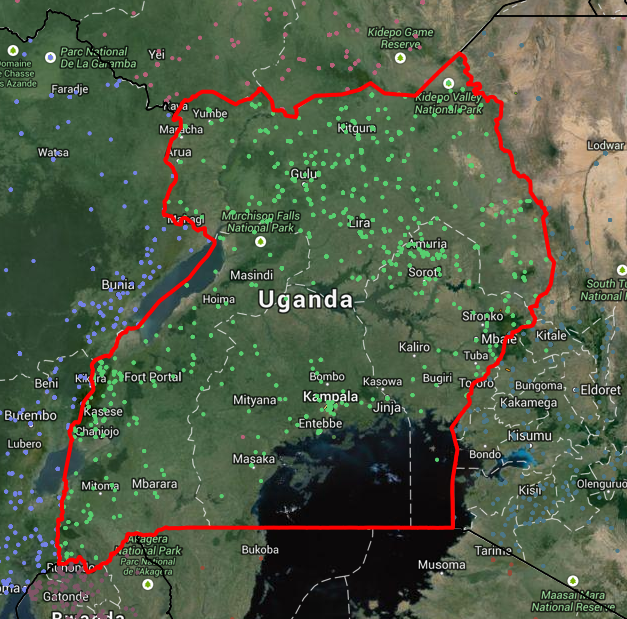
\includegraphics[width=\textwidth]{figures/uganda}
    \caption{Civil conflicts in Uganda 1997-2013.}
    \label{fig:map-points}
  \end{subfigure}~\begin{subfigure}[b]{0.5\textwidth}
    \centering
    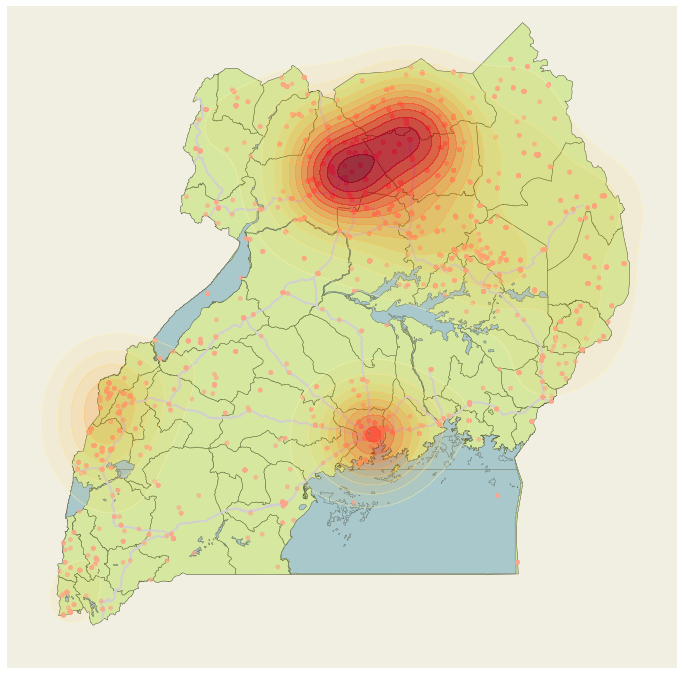
\includegraphics[width=\textwidth]{figures/map-with-smoothed-data}
    \caption{Conflicts with Mat\'{e}rn smoothing.}
    \label{fig:map-smoothed}
  \end{subfigure}
  \caption{Civil conflicts in Uganda.}
  \label{fig:map}
\end{figure}


\section{Modeling civil conflict}

\subsection{Events in space}

The violence and civil conflict events described in the ACLED dataset are coded with both a latitude and a longitude. One assumption we make is that these events are distributed due to underlying causes such as population centers, road access, historical land ownership, and other features that make conflicts more or less likely. It is difficult to directly create a generative model for these probabilities, so we will make the further assumption that the distribution of the data already incorporates and is representative of these factors. In effect, we treat the entire country of Uganda as a probability distribution from which geospatial conflict events could be sampled.  We took historical conflict location data from the entire ACLED data set and smoothed it using a Mat\'{e}rn covariance function.  Figure \ref{fig:map-smoothed} shows this smoothing applied to the same conflicts depicted in \ref{fig:map-points}.

We used this smooth function as a kernel-density esitmate (KDE). This estimate (i.e., the empirical distribution of the conflict data), has a complex functional form which makes it challenging to sample from. However, for any given coordinate it is quite simple to get the probability of an event. Given this property of our KDE, we can apply Monte Carlo sampling techniques to generate samples from this probability distribution. Visualizing the distribution, we can see that it is multi-modal with regions of low density between the modes. Because of these properties, we opted to use slice sampling to generate draws from the distribution. Figure \ref{fig:sampled-conflicts} shows the first 1,000 samples from this probability distribution.\footnote{We throw away samples that occur over water or outside of country boundaries.} Figure \ref{fig:histogram} shows the distribution of the samples as a two-dimensional histogram.

\begin{figure}
  \centering
  \begin{subfigure}[b]{0.5\textwidth}
    \centering
    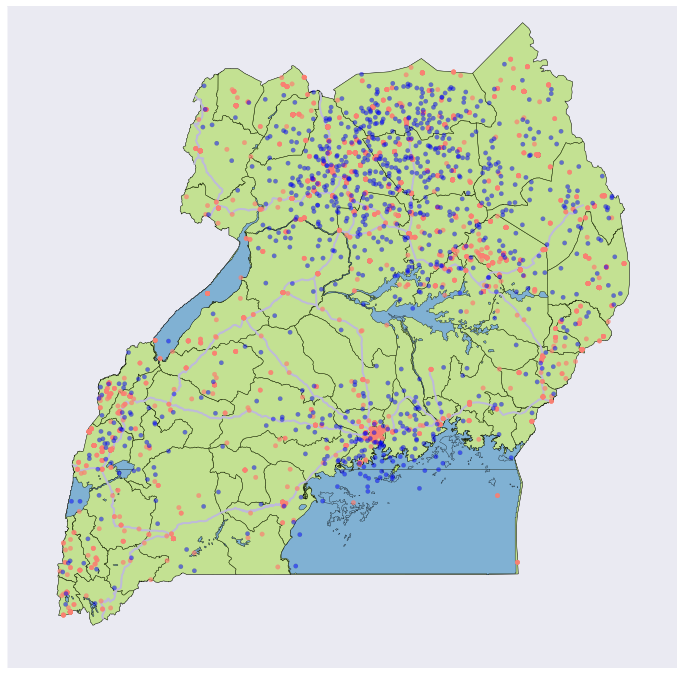
\includegraphics[width=\textwidth]{figures/1000-slice-samples}
    \caption{Blue dots are samples from the empirical distribution.}
    \label{fig:sampled-conflicts}
  \end{subfigure}~\begin{subfigure}[b]{0.5\textwidth}
    \centering
    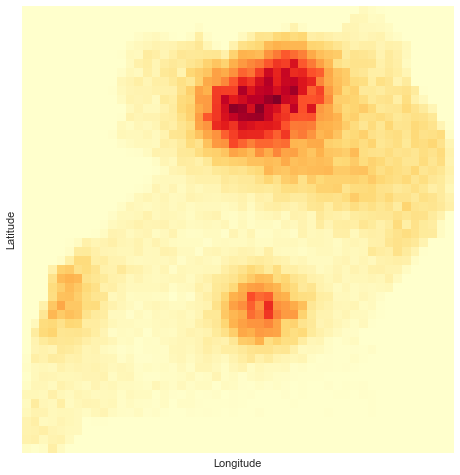
\includegraphics[width=\textwidth]{figures/histogram}
    \caption{2d histogram of slice samples from the empirical distribution.}
    \label{fig:histogram}
  \end{subfigure}
  \caption{Sampling from the empirical distribution.}
\end{figure}

When slice sampling, there are a number of parameter choices that are imporant. We want to choose our rectangle widths, burn-in, and thinning parameters appropriately. In testing, a thinning value of 10 reduced autocorrelation to less than 0.1 at a time lag of 1. We can see this result in Figure \ref{fig:autocorr}. We used the Gelman-Rubin potential scale reduction factor\cite{Gelman-Rubin} to determine if we were observing favorable mixing. Generally, a value less than 1.1 indicates good mixing. In both of our dimensions, the Gelman-Rubin statistic was less than this threshold. We also calculated the Geweke statistic, which is used to indicate convergence. A value less than 2 indicates convergence and for our draws, this statistic was $\ll$ 1. We can also examine convergence by looking at the trace plots for the samples. As we see in Figure \ref{fig:trace} these appear stationary.

\begin{figure}
  \centering
  \begin{subfigure}[b]{0.5\textwidth}
    \centering
    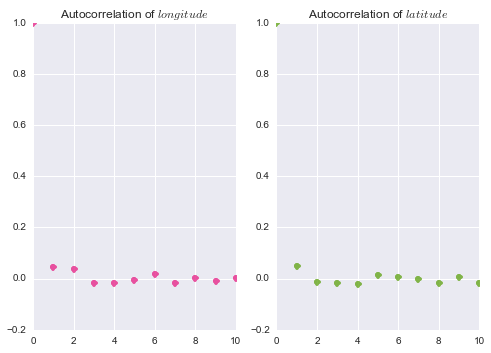
\includegraphics[width=\textwidth]{figures/autocorr-latlong}
    \caption{Autocorrelation for the samples from latitude and longitude}
    \label{fig:autocorr}
  \end{subfigure}
  \begin{subfigure}[b]{0.5\textwidth}
    \centering
    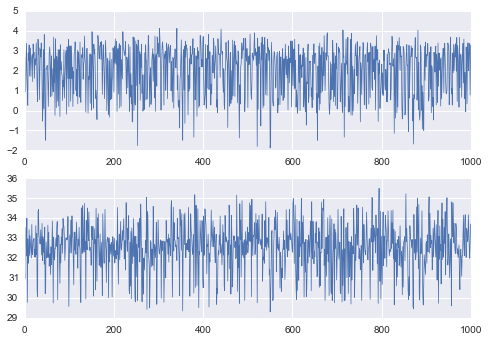
\includegraphics[width=\textwidth]{figures/trace-plots}
    \caption{Trace plots for draws from the latitude and longitude}
    \label{fig:trace}
  \end{subfigure}
  \caption{Diagnostic plots for location sampling.}
\end{figure}

\subsection{Events in time}
As a modeling assumption, we separate the dimensions of space and time as being independent. To model events in time across the country, we use an autoregressive Poisson GLM. While standard autoregressive models create a linear relation between a future value and a previous value, the Poisson GLM permits a linear relation between previous data and the mean of a Poisson distribution. This will allow us to retain the probabilistic interpretation of the events in time.

In order to model events using a Poisson distribution, we must discretize our time dimension. We opted for month-long increments. The thinking behind this decision is that we want to use sample draws to run our aid optimizations. If a model like this were to be used in planning for future conflicts, having a month-long window for a plan seems like a good balance between precision and logistic concerns.

The Autoregressive Poisson GLM model can be described as a log-linear relationship between the number of events of political violence and the mean of a Poisson distribution. We start with a timeseries, $\mathbf{X} = \{x_0, x_1,\hdots, x_N\}$, of $N$ counts of events at each discretized point in time. We also start with a lag $\Lambda$ that is the number of previous time steps to include in the model. We can now describe our features at time $t$ as the $\Lambda$ previous time steps: $\mathbf{X_{t, \Lambda}} = \{x_{t-\Lambda}, x_{t-\Lambda-1},\hdots, x_t\}$.

The linear predictor in the autoregressive model at a time step is $\eta_t$, and it is related to the mean of the Poisson distribution, $\mu_t$, by its canonical link function, $\log$.

\begin{align*}
\eta_t &= \mathbf{X}_{t, \Lambda}'\beta. \\
\mu_t &= \log(\eta_t) = \log(\mathbf{X}_{t, \Lambda}'\beta) \\
\end{align*}

Finally, the only parameter to the Poisson distribution is this mean, so the distribution of counts, $k$, at some time t+1 can be given by:

\begin{align*}
p(k | \mu_t) &= \frac{\mu_t^k}{k!}e^{-\mu_t} \\
p(k | \mathbf{X}_{t, \Lambda}, \beta) &= \frac{\log(\mathbf{X}_{t, \Lambda}'\beta)^k}{k!}e^{-\log(\mathbf{X}_{t, \Lambda}'\beta)} 
\end{align*}

We can fit this model by using Fisher scoring to calculate $\beta_\mathrm{MLE}$, the coefficients of the model. Figure \ref{fig:poisson} shows this model as compared to actual rates of conflict incidence.

\begin{figure}
\centering
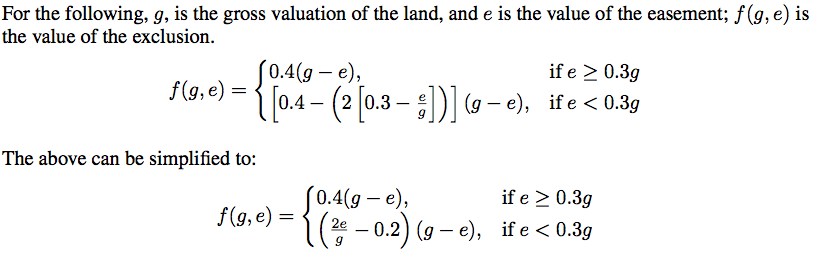
\includegraphics[width=\textwidth]{figures/poisson-regression.png}
\caption{The Poisson regression model.}
\label{fig:poisson}
\end{figure}

\subsection{Putting together the spatial and temporal}

We can now use our draws over space and time to generate a simulation of future conflicts in Uganda. These simulated scenarios will serve as the basis of our aid delivery optimization. The combination of modeling conflict events in space and time along with optimizing aid delivery could prove helpful to organizations such as the Red Cross in ordering supplies, allocating staff and volunteers, and developing infrastructure.

\section{Optimizing humanitarian aid delivery}

In the second part of this project, we use the temporal/geospatial conflict occurence model in the first section as both inspiration for the aid delivery analogy and also as a source of randomly sampled data points representing geospatially distributed conflicts.

\subsection{The traveling salesman problem}

One question of particular interest is how to route emergency aid
to locations where it is needed.  For concreteness, let's postulate a Red Cross medical or food supply caravan that originates from the organization's in-country headquarters. This caravan wishes to visit all $n$ emergent locations in order to
deliver needed supplies. They wish to do so in the most efficient manner possible.

This is the traveling salesman problem (TSP), an optimization problem that is quite well known. It was first described in 1932 by Karl Menger (shortly after his year here at Harvard as a visiting lecturer) and has been studied extensively ever since.\cite{Menger} Here is the traditional convex optimization specification of the problem:\cite{Winston}


\begin{align*}
\min &\sum_{i=0}^n \sum_{j\ne i,j=0}^nc_{ij}x_{ij} &&  \\
\mathrm{s.t.} & \\
	& x_{ij} \in \{0, 1\} && i,j=0, \cdots, n \\
	& \sum_{i=0,i\ne j}^n x_{ij} = 1 && j=0, \cdots, n \\
	& \sum_{j=0,j\ne i}^n x_{ij} = 1 && i=0, \cdots, n \\
	&u_i-u_j +nx_{ij} \le n-1 && 1 \le i \ne j \le n
\end{align*}

As is clear from the constraints, this is an integer linear program (ILP) where:

\begin{itemize}
  \item $x_{ij}$ is a binary decision variable indicating whether we go from location $i$ to location $j$.
  \item $c_{ij}$ is the distance\footnote{In our application, we deal with geospatial data on a large enough scale that the Euclidean distance is actually very imprecise. In order to model distances over the planet's surface, we use the Haversine formula.} between location $i$ and location $j$.
  \item The objective function is the sum of the distances for routes that we decide to take.
  \item The final constraint ensures that all locations are visited once and only once.
\end{itemize}

The problem, of course, is that brute force solution of the TSP is $\mathcal{O}$$(n!)$. Traditional, deterministic
algorithm approaches such as branch-and-bound or branch-and-cut are still impractical for larger numbers of nodes.
In many cases, exhaustive search for global optimality is not even particularly helpful as long as the solution
found is good enough. We will use simulated annealing (SA) to get acceptable solutions to the TSP.

Figure \ref{fig:routing-vanilla-tsp} shows a sample draw of conflict data (the blue points), and a near-optimal TSP route found through 50,000 iterations of simulated annealing.

\begin{figure}
  \centering
  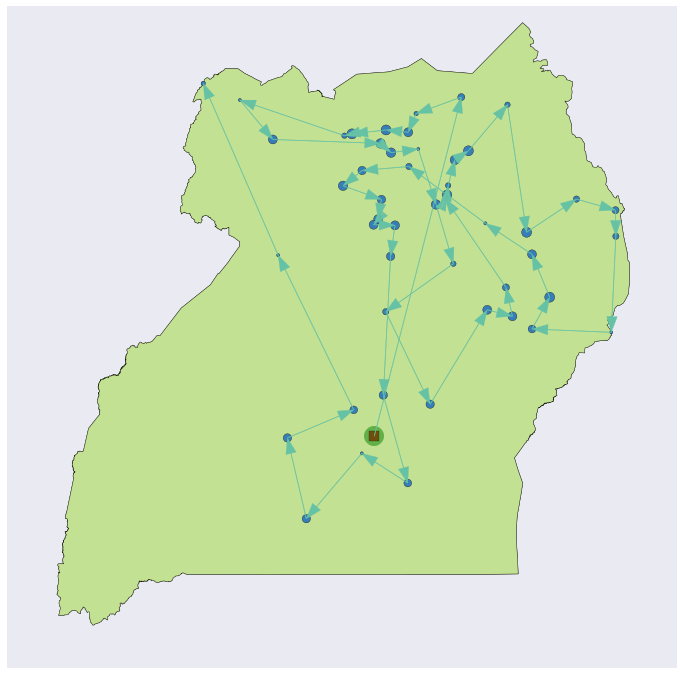
\includegraphics[width=\textwidth]{figures/routing-vanilla-tsp}
  \caption{Visiting all conflicts without reloading.}
  \label{fig:routing-vanilla-tsp}
\end{figure}

\subsection{Packing the aid truck --- the Knapsack Problem}

We extend the TSP into a multi-objective optimization problem
where \emph{the contents of the aid trucks} also have an optimization component. Therein lies
the knapsack problem: subject to a volume or weight constraint, and given that different locations
might have very different needs such as food, vaccinations, or emergent medical supplies, \emph{which
supplies do we pack on the trucks}?

Here's the unbounded\footnote{Often, this problem is formulated such that you can only bring one of each item, but that does not make sense in our application. Rather, we want to be able to bring as many types of each type of aid as we think necessary, and we'll assume that as many as desired are available to load on the trucks before starting out from HQ.} version of the knapsack problem:

\begin{align*}
\max &\sum_{i=1}^n v_i x_i &&  \\
\mathrm{s.t.} & \\
    & x_i \in \mathbb{Z} \\
    & x_i \geq 0 \\
	& \sum_{i=1}^n w_ix_i \leq W
\end{align*}

In this formulation:

\begin{itemize}
  \item $x_{i}$ is a zero or positive integer decision variable indicating how many units of item $i$
        we load on the truck.
  \item $v_i$ is the utility we get from bringing along item $i$.
  \item $w_i$ is the weight of item $i$.
  \item $W$ is the maximum weight the truck can carry.
\end{itemize}

\subsection{A brief detour for modeling assumptions}

Before we can optimize this aid delivery mechanism, we will need to decide a way to model humanitarian aid needs at a given conflict.

Let us assume that there are $K$ distinct types of humanitarian aid to be delivered. (Without loss of generality, we will use three categories for all of our examples --- perhaps we can think of them food aid, first aid supplies, and medicines for concreteness.) We can model each conflict's aid needs as

$$\boldsymbol x \sim \mathrm{Dir}(\boldsymbol \alpha)$$

where $\boldsymbol \alpha$ parameterizes the distribution to generate vectors of length $K$ representing the relative proportions of needs.\cite{Murphy} For example, in our three category example we might draw the vector $(0.11,\,0.66,\,0.23)$ for a certain conflict, meaning that 11\% of the aid needed at this conflict is food aid, 66\% is first aid supplies, and 23\% is medicines. Now that we know the proportions for the given conflict, how might we turn this unitless vector into absolute amounts?

For that reason, let's assign each conflict a scaled size $s \in [1, 10]$ based on the number of casualties (a proxy for the severity of the conflict). We can use this size scalar to turn our proportion vector into a vector of absolute needs.

It should be noted that \textbf{both of these modeling methods for proportions and size are ``plug-and-play''} --- because of purposely designed loose coupling in our model, these methods could trivially be replaced by a different method of calculating or predicting the needs of each conflict. For example, if an independent model was used to calculate each of $K$ needs based on the features of each conflict, those quantities could easily be plugged in to this model. Ultimately, the only quantities that our TSP/Knapsack model needs is an $n \times K$ matrix of aid needs for $n$ cities and $K$ categories of aid.

\subsection{A new objective function to integrate TSP and Knapsack}

For the vanilla TSP, we simply try to minimize the total distance. Now that we are adding a new objective, we will need to integrate the two into a coherent \textbf{loss function}.  Here is the function we will actually try to minimize in the combined TSP/Knapsack:

$$L(\boldsymbol x) = \text{total distance} + \text{sum of squared aid shortfalls}$$

The effect of squaring aid shortfalls acts as a weight, causing greater importance to be placed on minimizing this aspect of the problem first. Proposals wherein aid shortfalls occur are heavily penalized. As we will see in later graphs, once the SA algorithm is able to avoid all shortfalls and the concurrent massive loss function penalties, a much slower descent begins to take place wherein the distance is slowly optimized. See figure \ref{fig:sorties-loss} for a depiction of this phenomenon.

\subsection{Implementing the Knapsack aspect}

Figure \ref{fig:routing-reloading} shows the same draw of cities as in figure \ref{fig:routing-vanilla-tsp}, this time factoring in limited carrying capacity for aid supplies on the aid delivery mechanism and using our new loss function. As we can see, the huge penalty incurred when supplies run out quickly induces the simulated annealing algorithm to converge on a solution with multiple stops at HQ to reload.

\begin{figure}[h]
  \centering
  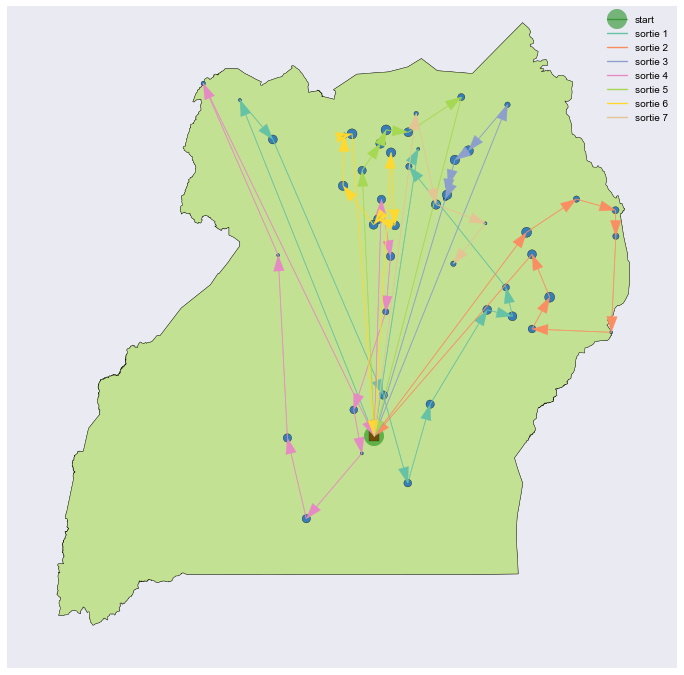
\includegraphics[width=\textwidth]{figures/routing-reloading}
  \caption{Routing with reloading from capital city Kampala.}
  \label{fig:routing-reloading}
\end{figure}

\begin{figure}[h]
  \centering
  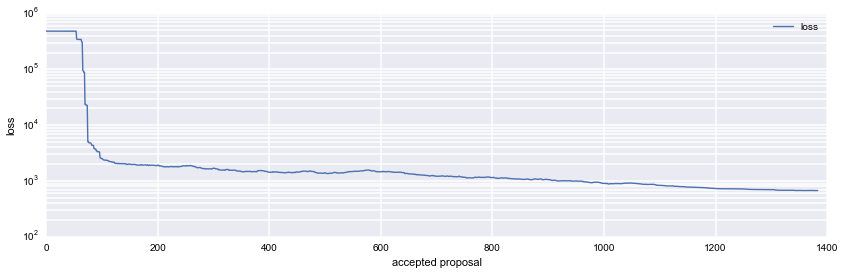
\includegraphics[width=\textwidth]{figures/sorties-loss}
  \caption{Loss function acceptances over 100,000 iterations.}
  \label{fig:sorties-loss}
\end{figure}

Figure \ref{fig:sorties} uses some uniformly distributed points on the $[0,50]$ plane to demonstrate how the proposed TSP/Knapsack routes converge as the number of iterations increases.


\begin{figure}[H]
  \centering
  \begin{subfigure}[b]{0.5\textwidth}
    \centering
    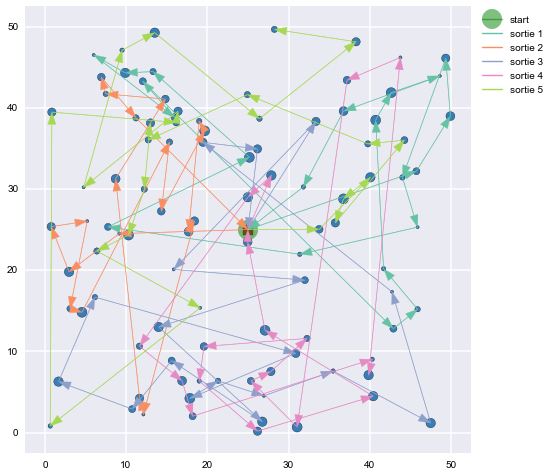
\includegraphics[width=\textwidth]{figures/sorties-5000}
    \caption{After 5,000 iterations.}
  \end{subfigure}~\begin{subfigure}[b]{0.5\textwidth}
    \centering
    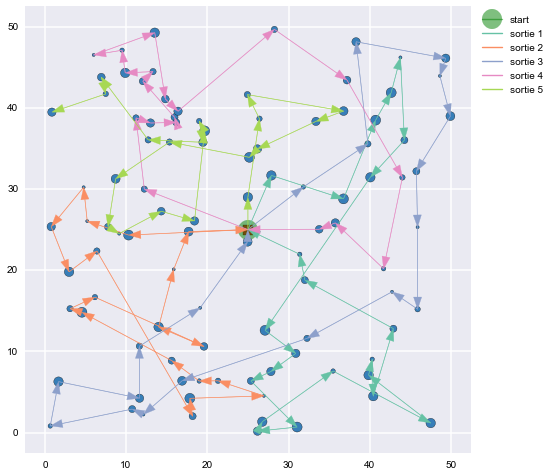
\includegraphics[width=\textwidth]{figures/sorties-20000}
    \caption{After 20,000 iterations.}
  \end{subfigure}
  \begin{subfigure}[b]{\textwidth}
    \centering
    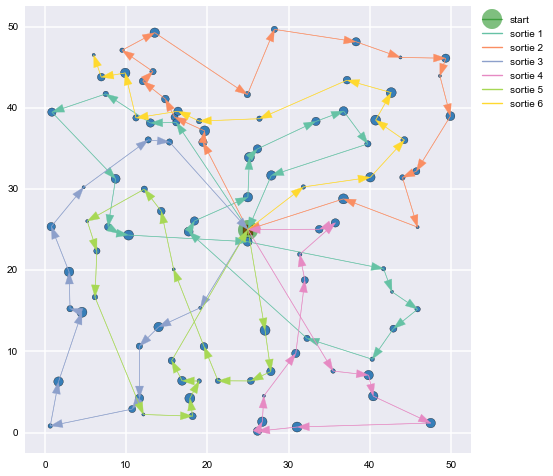
\includegraphics[width=0.75\textwidth]{figures/sorties-100000}
    \caption{After 100,000 iterations.}
  \end{subfigure}
  \caption{Example routing for the TSP/Knapsack hybrid using uniformly distributed points.}
  \label{fig:sorties}
\end{figure}

\subsection{Finding the optimal site for the resupply location}

Our initial assumption was that the HQ was located in the capital city of Kampala. However, we should ask whether our HQ could be more conveniently located. We can answer this question by treating the reload location as another parameter and continuing to sample HQ locations using SA. Figure \ref{fig:routing-reloading-hq-optimal} shows the TSP/Knapsack optimized once again, this time using a the optimal HQ location, while \ref{fig:comparative-loss-plot} compares the loss function as each method converges to its best possible configuration.

\begin{figure}
  \centering
  \begin{subfigure}[b]{0.5\columnwidth}
    \centering
    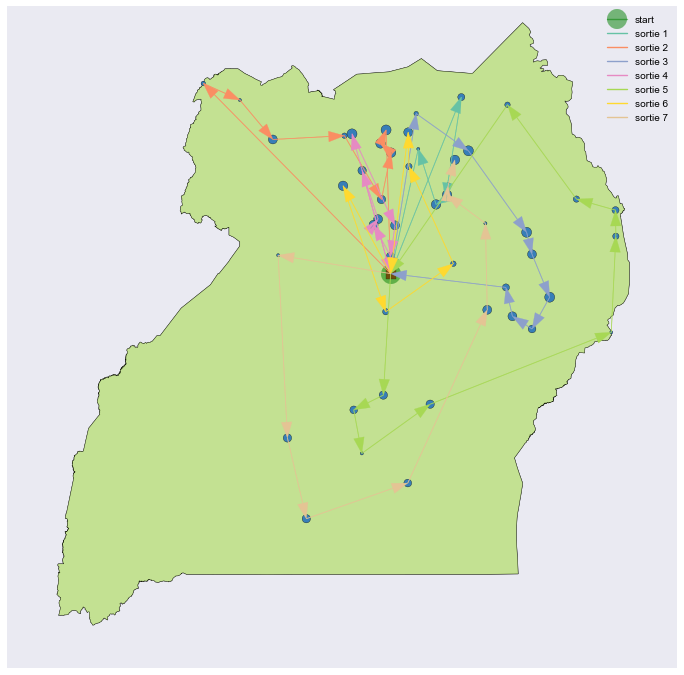
\includegraphics[width=\textwidth]{figures/routing-reloading-hq-optimal}
    \caption{Routing with reloading from optimal HQ.}
    \label{fig:routing-reloading-hq-optimal}
  \end{subfigure}~\begin{subfigure}[b]{0.46\columnwidth}
    \centering
    \centering
    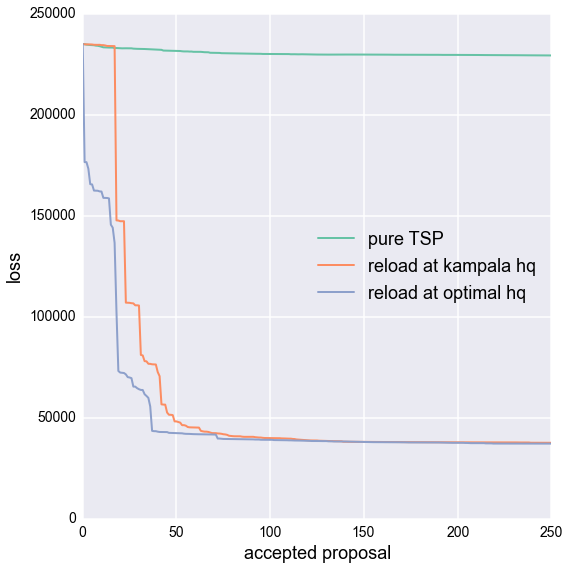
\includegraphics[width=\textwidth]{figures/comparative-loss-plot}
    \caption{Example loss function optimization convergence for $n=50$.}
    \label{fig:comparative-loss-plot}
  \end{subfigure}
  \caption{Optimizing aid delivery routing with reloading.}
\end{figure}

\section*{Conclusions}

In each part of this problem, analytical solutions either do not exist (e.g. in the distribution of events) or are computationally infeasible (e.g. in the TSP/Knapsack optimizations).  We found that using a metaheuristic such as SA converged on robust solutions in relatively short order. In the future, we would like to formulate our loss function based on real world data based on refugee locations and aid distribution requirements; our methodology would not change, but the solutions would be more useful for predictive tasks. Additionally, the separate models could be fit and incorporated which realistically model how much of each type of aid is needed at each conflict location. Future research might also include adding many more constraints or twists to the problem, and trying different stochastic optimization techniques such as genetic algorithms, Tabu search, or ant colony optimization.


\bibliography{proposal}

\end{document}
